\documentclass[a4paper]{article}

\usepackage{INTERSPEECH2016}

\usepackage{graphicx}
\usepackage{amssymb,amsmath,bm}
\usepackage{textcomp}

\def\vec#1{\ensuremath{\bm{{#1}}}}
\def\mat#1{\vec{#1}}

% Ilaria: I had to add the following commands: a pandoc command which was causing problems when using \tightlist (solution found here: https://github.com/jgm/pandoc-templates/blob/master/default.latex); this command is also found in the LaTex output created by RStudio.
\providecommand{\tightlist}{% 
\setlength{\itemsep}{0pt}\setlength{\parskip}{0pt}}
% and five packages:
\usepackage{url}
\usepackage{hyperref}
\usepackage{longtable}
\usepackage{booktabs}
\usepackage{supertabular}

% Ilaria: The original pandoc output uses \longtable to generate the table from Markdown; in order to correctly generate it in this template, I had to add the following code (found in http://tex.stackexchange.com/questions/161431/how-to-solve-longtable-is-not-in-1-column-mode-error)
\makeatletter
\let\oldlt\longtable
\let\endoldlt\endlongtable
\def\longtable{\@ifnextchar[\longtable@i \longtable@ii}
\def\longtable@i[#1]{\begin{figure}[t]
\onecolumn
\begin{minipage}{0.5\textwidth}
\oldlt[#1]
}
\def\longtable@ii{\begin{figure}[t]
\onecolumn
\begin{minipage}{0.5\textwidth}
\oldlt
}
\def\endlongtable{\endoldlt
\end{minipage}
\twocolumn
\end{figure}}
\makeatother
% End of longtable addition

\sloppy % better line breaks
\ninept

\title{FinalMD}

%%%%%%%%%%%%%%%%%%%%%%%%%%%%%%%%%%%%%%%%%%%%%%%%%%%%%%%%%%%%%%%%%%%%%%%%%%
%% If multiple authors, uncomment and edit the lines shown below.       %%
%% Note that each line must be emphasized {\em } by itself.             %%
%% (by Stephen Martucci, author of spconf.sty).                         %%
%%%%%%%%%%%%%%%%%%%%%%%%%%%%%%%%%%%%%%%%%%%%%%%%%%%%%%%%%%%%%%%%%%%%%%%%%%
\makeatletter
\def\name#1{\gdef\@name{#1\\}}
\makeatother
\name{{\em Ilaria Torre, Frank Loesche}}
%%%%%%%%%%%%%%% End of required multiple authors changes %%%%%%%%%%%%%%%%%

\makeatletter
\def\name#1{\gdef\@name{#1\\}}
\makeatother \name{{\em Ilaria Torre$^1$, Frank Loesche$^1$}}

\address{$^1$Plymouth University \\
{\small \tt ilaria.torre@plymouth.ac.uk, frank.loesche@plymouth.ac.uk}
}

%\twoauthors{Karen Sp\"{a}rck Jones.}{Department of Speech and Hearing \\
%  Brittania University, Ambridge, Voiceland \\
%  {\small \tt Karen@sh.brittania.edu} }
%  {Rose Tyler}{Department of Linguistics \\
%  University of Speechcity, Speechland \\
%  {\small \tt RTyler@ling.speech.edu} }

%
\begin{document}

  \maketitle
  %
  \section{Header 1}\label{header-1}
  
  This is some very basic text.
  
  \subsection{Header 2}\label{header-2}
  
  This is some other text in a sub-heading. You can go on until level 6.
  
  Newlines are interpreted as new paragraphs.
  
  I can emphasize text like \emph{this} or like \textbf{this}.
  
  Unordered lists are created with symbols like *, -, +\ldots{} but the
  first item of the list needs to be preceded by an empty line:
  
  \begin{itemize}
  \tightlist
  \item
    I like cooking
  \item
    I also like languages
  \item
    and I like folk music
  
    \begin{itemize}
    \tightlist
    \item
      especially Blackbeard's Tea Party!
    \end{itemize}
  \end{itemize}
  
  Ordered lists are created with numbers and dots. Even if you mess up the
  numbering, MD will fix it for you:
  
  \begin{enumerate}
  \def\labelenumi{\arabic{enumi}.}
  \tightlist
  \item
    Item 1
  \item
    Item 2
  \item
    Item 3
  \end{enumerate}
  
  Links can be added in text like this:
  \href{http://www.blackbeardsteaparty.com/}{click here} or like this:
  \url{http://www.blackbeardsteaparty.com/}
  
  Images are basically links, but they have to be also separated from the
  main text by an empty line before and after:
  
  \begin{figure}[htbp]
  \centering
  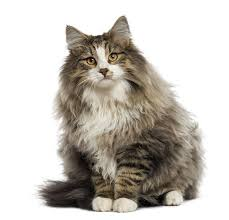
\includegraphics{images/fluffycat.jpg}
  \caption{A super fluffy cat}
  \end{figure}
  
  
  Tables can be written with -- and \textbar{}\textbar{} symbols:
  
  \begin{longtable}[]{@{}lcr@{}}
  \toprule
  Tables & Are & Cool\tabularnewline
  \midrule
  \endhead
  col 3 is & right-aligned & \$1600\tabularnewline
  col 2 is & centered & \$12\tabularnewline
  zebra stripes & are neat & \$1\tabularnewline
  \bottomrule
  \end{longtable}
  
 
 \subsection{R Markdown}\label{r-markdown}
 
 This is an R Markdown document. Markdown is a simple formatting syntax
 for authoring HTML, PDF, and MS Word documents. For more details on
 using R Markdown see \url{http://rmarkdown.rstudio.com}.
 
 When you click the \textbf{Knit} button a document will be generated
 that includes both content as well as the output of any embedded R code
 chunks within the document. You can embed an R code chunk like this:
  
%this is the output from pandoc, but we can eliminate these lines (I will just comment them out)    
%    \begin{Shaded}
%    \begin{Highlighting}[]
%    \KeywordTok{summary}\NormalTok{(cars)}
%    \end{Highlighting}
%    \end{Shaded}
    
    \begin{verbatim}
    ##      speed           dist       
    ##  Min.   : 4.0   Min.   :  2.00  
    ##  1st Qu.:12.0   1st Qu.: 26.00  
    ##  Median :15.0   Median : 36.00  
    ##  Mean   :15.4   Mean   : 42.98  
    ##  3rd Qu.:19.0   3rd Qu.: 56.00  
    ##  Max.   :25.0   Max.   :120.00
    \end{verbatim}
    
  %\newpage 
  %\eightpt
  %\bibliographystyle{IEEEtran}

  %\bibliography{MyBibliography.bib} %you can add your bibliography here; change this to the name of your bibliography file
  
  
  

%  \begin{thebibliography}{9}
%    \bibitem[1]{Davis80-COP}
%      S.\ B.\ Davis and P.\ Mermelstein,
%      ``Comparison of parametric representation for monosyllabic word recognition in continuously spoken sentences,''
%      \textit{IEEE Transactions on Acoustics, Speech and Signal Processing}, vol.~28, no.~4, pp.~357--366, 1980.
%    \bibitem[2]{Rabiner89-ATO}
%      L.\ R.\ Rabiner,
%      ``A tutorial on hidden Markov models and selected applications in speech recognition,''
%      \textit{Proceedings of the IEEE}, vol.~77, no.~2, pp.~257-286, 1989.
%    \bibitem[3]{Hastie09-TEO}
%      T.\ Hastie, R.\ Tibshirani, and J.\ Friedman,
%      \textit{The Elements of Statistical Learning -- Data Mining, Inference, and Prediction}.
%      New York: Springer, 2009.
%    \bibitem[4]{YourName16-XXX}
%      F.\ Lastname1, F.\ Lastname2, and F.\ Lastname3,
%      ``Title of your INTERSPEECH 2016 publication,''
%      in \textit{Interspeech 2016 -- 16\textsuperscript{th} Annual Conference of the International Speech Communication Association, September 8–12, San Francisco, California, USA, Proceedings, Proceedings}, 2016, pp.~100--104.
%  \end{thebibliography}

\end{document}
